\chapter{State of the Art} \label{ch:StateOfTheArt}

This chapter covers the state of the art in heterogenous computing programming models, with a focus on Graphic Processing Units (GPUs). 

Today, over six hundred applications utilize GPU acceleration across a broad range of industries including: finance, design for manufacturing/construction, artificial intelligence, medical imaging and more. As such, it was a very important platform to add to the MANGO software stack, and one of the main contributions of our thesis.

Section \ref{sect:history-gpgpu} covers the history of advancements in GPGPU technology and is largely based on \cite{brief_history_gpgpu}, a talk by Nvidia Software Engineer Mark Harris. This is a very interesting topic and shows the evolution in development using GPUs, culminating in the release of Nvidia's CUDA. 

The following sections cover other programming models starting from OpenCL in section \ref{sect:opencl}. It being the most well established programming model in GPUs after CUDA, which also provides support for programming in CPUs and FPGAs.

ROCm, AMD's response to the significant adoption of CUDA, is covered in section \ref{sect:rocm}. By adopting a very similar API to CUDA, AMD is able to easily port existing CUDA applications in order to run them on their own GPUs while still being able to compile for Nvidia's.

After that, section \ref{sect:openmp-openacc} covers both OpenMP and OpenACC, which adopt a very similar compiler-directive-based approach to programming GPUs.

Finally, sections \ref{sect:sycl} and \ref{sect:kokkos} cover SYCL and Kokkos respectively. SYCL being the latest open standard for heterogeneous computing, which aims at providing a higher level approach than OpenCL. On the other hand, Kokkos works towards abstracting away the memory access patterns needed by different architectures in such a way that the same code can exhibit the best performing one depending on the target device.

\section{The History of GPGPU} \label{sect:history-gpgpu}

\subsection{Inception}
The first documented case of computation on a graphics processor dates to June 1985, when Tim Van Hook implemented the world's first GPU ray-tracing on the Ikonas RDS-3000 \cite{ikonas}. Van Hook followed this up the next year with a paper on solid modelling with the Ikonas \cite{solid_modeling_ikonas}.

In August 1999, Kedem et al. \cite{unix_passwords_gpgpu} published a paper where they used experimental graphics engine PixelFlow to perform a brute force attack on Unix passwords. PixelFlow was a heterogeneous parallel machine used for high-speed and high-quality image generation. For their research, PixelFlow was setup with 18 SIMD arrays, each one with 8K processing elements (PE) for a total of 144K (147,456) PEs running at 100Mhz. The machine had some performance problems for this application due to the limited instruction set, which was focused on image computations. Because of this, the results were poorer than expected. It was calculated that the machine would be able to check all lowercase passwords (28.9\% of passwords at the time) in 3.19 hours.

\begin{figure}[h]
    \centering
    
\includegraphics[width=0.5\textwidth]{img/voronoi.png}
    \captionsetup{justification=centering}
    \caption{Generalized Voronoi diagram computed interactively on PC (Credit: Hoff et al.)}
\end{figure}

Also in 1999, Hoff et al. \cite{voronoi_diagrams_gpgpu} managed to perform computations of generalized Voronoi diagrams using graphics accelerators, such as the Nvidia TNT2, connected to a PC \cite{brief_history_gpgpu}, as opposed to the specialized hardware in the PixelFlow. This was achieved by using the OpenGL API \cite{opengl}. However, at that time GPUs were not programmable. The hardware exposed what is known as a Fixed Function Pipeline which the user could configure according to their needs. With that configuration, the GPU would execute a series of built in math functions which were focused on rendering, not on computation \cite{opengl_fixed_function_pipeline}.

\subsection{Programmable GPUs}
Programmable GPUs did not come until 2001, as Nvidia introduced GeForce series 3. This replaced the fixed functions in the previous model with programmable shaders which could be controlled by the developers \cite{nvidia_nfinitefx_pixel, nvidia_nfinitefx_vertex}. These features were, of course, aimed at game developers and 3D designers, but they also allowed for new applications of GPU technology.

Using a GeForce 3, Larsen and McAllister achieved the first matrix multiplication done on a GPU \cite{early_matrix_multiplication_gpgpu}. Their work was done by mapping the matrices into textures that could be manipulated with the OpenGL API. This textures would be transferred to the GPU, rendered and then copied back to CPU memory to be mapped again to a matrix format so results could be read. Incidentally, the resulting "matrix texture" would be shown on screen. There is no explicit mention of the use of programmable shaders in this work, however this would not have changed the study drastically as the fixed functions of the previous model could handle the operations required. The main problem Larsen and McAllister found was the 8 bit fixed point precision and saturation arithmetic used by the hardware. Saturation arithmetic, although very useful in graphics, makes it harder to design a higher precision fixed-point implementation.

Approximate simulations of natural phenomena were achieved on the GPU by Harris et al. \cite {physics_simulations_gpgpu}. This included interactive visualizations of convection, reaction-diffusion and boiling. As the end effect of the simulation was to display visuals, this application had the advantage that data did not need to be transferred back to the CPU once results were computed. Again, during these experiments the most problematic aspect was the precision of the fixed-point operations. This contributed to more difficult programmability and arithmetic errors. During this work, the researchers exploited the programming capabilities of the GeForce 3 and, at the time, newly released GeForce 4. ATI had also released a programmable GPU in the form of the Radeon 8500, which promised to add more power to the simulations, however the system was not ported to it at the time of publication.

In late 2002, after seeing the growing trend in general purpose computation on GPUs, Harris coined the term GPGPU, an acronym for "General Purpose computing on Graphics Processing Units" \cite{brief_history_gpgpu}. GPGPU.org, a website dedicated to news and resources on GPGPU research, would go live August 2003.

DirectX 9 (DX9) introduced the Shader Model 2.0 and with it support for floating-point operations. In July 2002, ATI released the first DirectX 9 capable graphics card in the form of the Radeon 9700 PRO \cite{ati_9700_pro}. Nvidia followed up with their own DX9 GPU, the GeForceFX, in January 2003 \cite{geforcefx}.

DX9 Hardware allowed researchers to implement algorithms which previously could not be ran on the GPU due to lack of floating-point support. One example of this is global illumination. In \cite{photon_mapping_gpgpu}, Purcell et al. achieve interactive frame rates on a GeForce FX 5900 computing global illumination via photon mapping. This is done by utilizing an incremental approach, where increasingly better approximations are rendered until the image converges, the initial approximations can be shown to the user for interactive feedback. On a 160 x 160 window, it is possible to interactively manipulate the camera, scene geometry and light source. Once interaction stops, the illumination converges in one or two seconds, an example can be seen in figure \ref{fig:lighting-approximations}.

\begin{figure}[ht]
    \centering
    \begin{tabular}{ccc}
        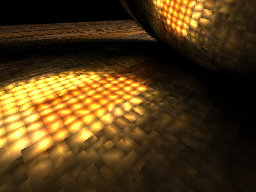
\includegraphics[width=0.3\textwidth]{img/half-second-glass-ball.png} & 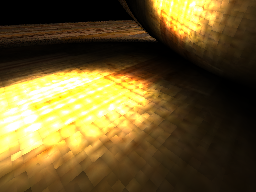
\includegraphics[width=0.3\textwidth]{img/one-second-glass-ball.png} & 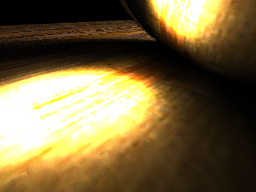
\includegraphics[width=0.3\textwidth]{img/two-second-glass-ball.png} \\
        (a) 0.5s                                                              & (b) 1.0s                                                             & (c) 2.0s
    \end{tabular}
    \captionsetup{justification=centering}
    \caption{Lighting approximations over time (Credit: Purcell et al.)}
    \label{fig:lighting-approximations}
\end{figure}

The main bottleneck that Purcell et al. faced in their paper stemmed from the lack of random access writes. While the original photon mapping algorithm uses a balanced k-d tree, it is not possible to construct one on the GPU due to this limitation. Instead, the researchers had to modify the algorithm in order to account for this, replacing the k-d tree with a uniform grid. To build this grid, they implemented two algorithms, bitonic merge sort and stencil routing. The bitonic sort is computationally less efficient, needing \(O(\log^2 n)\) rendering passes. On the other hand, stencil routing can be computed in a single pass but suffers from memory readback performance bottlenecks.

All the kernels were written in Cg, a general purpose language for GPUs released by Nvidia at the start of 2003 \cite{nvidia_cg}. The design of Cg was inspired by the C language to provide a high level language that is still close to the underlying hardware. The C syntax served as a starting point which was then extended and modified as necessary to support GPU architectures effectively. The general purpose nature of the language allows the programmer to use very similar code to program the vertex and fragment stages of the rendering pipeline. This also simplifies programming for GPGPU applications, an aspect that was taken into account when designing the language due to the rising popularity of the field.

\subsection{Brook}
Languages like Cg, Microsoft's HLSL and OpenGL's GLslang allowed for shaders to be written in C-like syntax. However, they still required the programmer to express GPU applications in terms of graphics primitives and to use the existing graphics APIs to control the rest of the graphics pipeline, such as memory allocation and loading programs. In August 2004 researchers at Stanford University presented Brook \cite{brook}, a programming environment that provides developers with a view of the GPU as a streaming coprocessor.

Instead of working with textures and shaders, the Brook language allows the programmer to think in terms of streams and kernels. A stream is a collection of records (elements) and is denoted by angle-brackets, i.e. \texttt{float x<100>}. Access to streams is limited to kernels and the \texttt{streamRead} and \texttt{streamWrite} operators, which transfer memory between memory and streams. A kernel is a function that performs parallel operations over one or more streams. Calling a kernel on a stream performs an implicit loop over the elements of the stream, invoking the body of the kernel for each element. An example Brook snippet can be seen in listing \ref{lst:brook_saxpy}.

\begin{lstlisting}[style=BrookStyle, caption=Brook saxpy example, float, floatplacement=H, label={lst:brook_saxpy}]
kernel void saxpy(float a, float4 x<>, float4 y<>, out float4 z<>) {
    z = a*x + y;
}

void main(void) {
    float a;
    float4 X[100], Y[100], Z[100];
    float4 x<100>, y<100>, z<100>;
    // Omitted: Initialize a, X, Y
    streamRead(x, X);     // copy data from mem to stream
    streamRead(y, Y);
    saxpy(a, x, y, z);    // execute kernel on all elements
    streamWrite(z, Z);    // copy data from stream to mem
}   
\end{lstlisting}

A kernel accepts different types of arguments:

\begin{itemize}
    \item Input streams that contain read-only data for kernel processing.
    \item Output streams (marked with the \texttt{out} keyword) that store the result of a kernel computation.
    \item Gather streams which are declared as a C array with brackets, i.e. \texttt{gather[]}. A gather stream allows for arbitrary indexing of its elements.
    \item Non-stream arguments, which are read-only constants.
\end{itemize}

Due to the same GPU limitations experienced by Purcell et al., Brook does not provide arbitrary writes, only arbitrary reads with the gather streams.

The Brook compilation and runtime system maps the language onto existing programmable GPU APIs, including OpenGL and DirectX. The system consists of two components: \texttt{brcc}, a source-to-source compiler and the Brook Runtime (BRT), a library that provides runtime support for kernel execution. \texttt{brcc} maps Brook kernels into Cg shaders which are then translated into GPU assembly by vendor-provided shader compilers. Additionally, it emits C++ code which uses BRT to invoke the kernels.

\subsection{The Unified Shader Model}

In November 2005, Microsoft launched the XBOX 360 console. A noteworthy aspect of this launch is that the console used the first unified shader architecture GPU on the market, the ATI Xenos \cite{xbox_360_specs}. Previously, GPUs had different processing units which either handled vertex or fragment shader operations. In the unified shader model, there is a single type of unit, called shader core, which can handle both type of operations. The main selling point of this change is that greater flexibility allowed for all the units to be used during rendering, no matter the type of workload. With the classical fixed shader model, heavy polygon scenes would leave the fragment units idle, while heavy pixel scenes would underutilize the vertex units. This issue is illustrated in figure \ref{fig:gpu-fixed-shader-perf}. Figure \ref{fig:gpu-unified-shader-perf} shows how the unified shader model is able to better utilize the available resources.

\begin{figure}[ht]
    \centering
    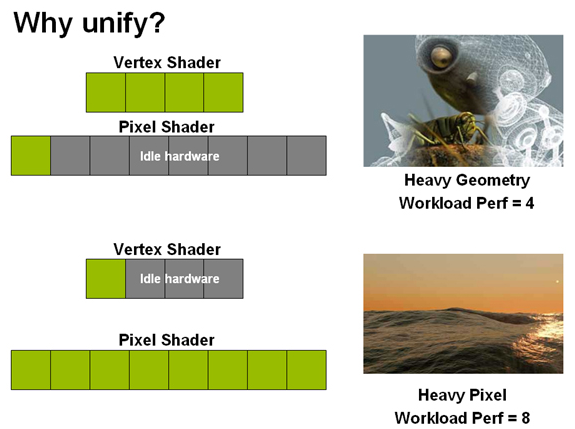
\includegraphics[width=0.6\textwidth]{img/classic-model-gpu-idle-units.png}
    \captionsetup{justification=centering}
    \caption{Fixed shader model performance characteristics (Credit: Nvidia)}
    \label{fig:gpu-fixed-shader-perf}
\end{figure}

\begin{figure}[ht]
    \centering
    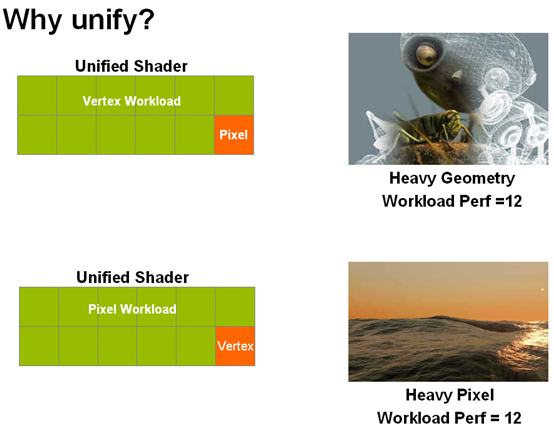
\includegraphics[width=0.6\textwidth]{img/unified-shader-gpu-utilization.png}
    \captionsetup{justification=centering}
    \caption{Unified shader performance characteristics (Credit: Nvidia)}
    \label{fig:gpu-unified-shader-perf}
\end{figure}

While ATI produced the first unified shader GPU for the XBOX 360, Nvidia was the one  to release the model in PCs with the GeForce 8800 in November 2006. DirectX 10 had introduced Shader Model 4.0 which included a unified shader instruction set. Even though a unified architecture was not a requirement to use DirectX 10, it provided better efficiency, load-balancing and power utilization \cite{geforce_8800_architecture}. A block diagram of the GeForce 8800 can be seen in figure \ref{fig:8800-arch}. The streaming processors (SP) marked in green are the units in charge of all the shader processing (the shader cores).

\begin{figure}[ht]
    \centering
    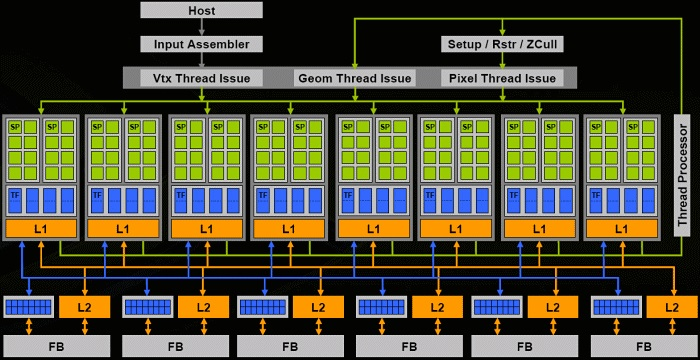
\includegraphics[width=\textwidth]{img/geforce-8800-block-diagram.png}
    \captionsetup{justification=centering}
    \caption{GeForce 8800 GTX Block Diagram (Credit: Nvidia)}
    \label{fig:8800-arch}
\end{figure}

\subsection{AMD Close To The Metal}

ATI (from here on out referred to as AMD due to their acquisition in 2006) was also the first vendor to release direct support for GPGPU with its CTM or "Close To The Metal" system in late 2006. CTM provides raw assembly level access with its hardware abstraction layer (HAL). The compute abstraction layer (CAL) adds higher level constructs and a C API, however this only covers context, memory management and kernel execution, the kernel itself must still be written in a low level AMD intermediate representation \cite{amd_ctm_programming_guide}. For higher level programming, AMD also supported compilation of Brook programs directly to the hardware \cite{gpu_computing}.

By providing a first party computing model, CTM eliminates the need for developers to work with graphics APIs and deal with a rendering pipeline. Instead of having to adapt algorithms work with textures, vertices, pixels and shaders, the developer can perform computation by binding memory as inputs and outputs to the stream processors directly. This includes Brook, which no longer has the requirement to work on top of a graphics API backend.

\subsection{Nvidia CUDA} \label{STATE:cuda}

In June of 2007, Nvidia introduced CUDA \cite{cuda_toolkit_archive}. The significant redesign that came with the adoption of unified shaders for the GeForce 8800 GTX, as well as the flexibility achieved by the final model, allowed Nvidia to develop a hardware and software solution for data-intensive computing.

The CUDA C++ language is a minimal extension over C++ adding parallelism features. As opposed to AMD CTM, which combined the CAL C API with a low level kernel language, this programming model is single source. CPU (host) code and GPU (kernel) code are written in the same language and can be contained in the same file. When launching a kernel in CUDA, the user must provide an \textit{execution configuration} with a custom $<<< ... >>>$ syntax. The most important aspect of this configuration is the dimensions of the \textit{grid} and \textit{thread blocks}.

A thread block is a group of threads that is executed in a single streaming multiprocessor (SM), which is a group of stream processors (SP). As its definition indicates, a thread block must fit in a single SM and thus is limited by the hardware. Currently, this limits a thread block to contain a maximum of 1,024 threads. The dimensions of a thread block is given by a \texttt{dim3} which is a 3-dimensional vector, allowing the programmer to distribute the threads in a 3D configuration. Using 1D, 2D or 3D configurations is purely for convenience of the developer. They can use the one that best suits the kernel to run.

A grid is then a group of thread blocks. The maximum amount of blocks that can run in parallel is limited by the amount of SMs in a particular GPU, however this does not limit the dimensions of the grid. Due to memory latency, it is better to launch a large grid of blocks at the same time. Having a lot of blocks at its disposal allows the GPU to switch the blocks being executed depending on the contents of the memory. If a given block needs to load a piece of data from memory as it is not currently in the GPU registers, it can be swapped out until the data is loaded, hiding the overhead. Grid dimensions are also indicated with a \texttt{dim3}, for the same reasons as the blocks.

When running a kernel, the CUDA runtime assigns a unique ID to each execution of the kernel, according to its theoretical place in the grid and the block. On the device side, the programmer can query the block and thread ids as well as the block and thread dimensions in order to handle different sections of the data. 

An example of CUDA code can be seen in listing \ref{lst:cuda_saxpy}.

When compared to AMD's offering, CUDA is a higher level interface than CAL, but it also provides more hardware access than Brook. In exchange for requiring more hardware knowledge, CUDA exposes multiple levels of memory hierarchy, per-thread registers, fast shared memory between threads in a block, board memory and host memory. In addition, while Brook only exposes a single dimension of parallelism, data parallelism via streaming, CUDA provides data parallelism and multithreading. CUDA kernels are also more flexible, as they allow the use of pointers, arbitrary writes and thread synchronization between threads in a single block \cite{gpu_computing}.

\begin{lstlisting}[style=CStyle, caption=CUDA saxpy example, float, label={lst:cuda_saxpy}]
__global__ void saxpy(int n, float a, float *x, float *y, float *z) {
  int i = blockIdx.x * blockDim.x + threadIdx.x;
  if (i < n) z[i] = a * x[i] + y[i];
}

int main(void) {
  float a;
  float X[100], Y[100], Z[100];
  float *d_x, *d_y, *d_z;

  // Omitted: Initialize a, X, Y

  cudaMalloc(&d_x, 100 * sizeof(float)); 
  cudaMalloc(&d_y, 100 * sizeof(float));
  cudaMalloc(&d_z, 100 * sizeof(float));

  cudaMemcpy(d_x, X, 100 * sizeof(float), cudaMemcpyHostToDevice);
  cudaMemcpy(d_y, Y, 100 * sizeof(float), cudaMemcpyHostToDevice);
  cudaMemcpy(d_z, Z, 100 * sizeof(float), cudaMemcpyHostToDevice);

  // Launch kernel in a single block of 256 threads
  saxpy<<<1, 256>>>(100, a, d_x, d_y, d_z);

  cudaMemcpy(Z, d_z, 100 * sizeof(float), cudaMemcpyDeviceToHost);

  cudaFree(d_x);
  cudaFree(d_y);
  cudaFree(d_z);
}
\end{lstlisting}

Overall, CUDA's advantages over AMD's CTM gave Nvidia the upper hand in the GPGPU field and it is still in use to this day. By contrast, in 2008, AMD's CTO of graphics announced that the company was shifting its focus away from CTM and into the upcoming OpenCL standard \cite{amd_ctm_ditch}, detailed in the following section.

\section{OpenCL} \label{sect:opencl}

Released in December 2008, Open Compute Language or OpenCL \cite{opencl_spec} is an open industry standard for programming a heterogeneous collection of CPUs, GPUs and other discrete computing devices organized into a single platform. It provides a framework for parallel programming and includes a language, API, libraries and a runtime system to support software development. By leveraging OpenCL, an application can use a host and one or more OpenCL devices as a single heterogeneous parallel computer system.

The framework is comprised by the following components:
\begin{itemize}
    \item \textbf{Platform layer}: Allows the host program to create contexts and discover OpenCL devices and their capabilities.
    \item \textbf{Runtime}: Allows the host program to manipulate contexts one they have been created.
    \item \textbf{Compiler}: Creates program executables that contain OpenCL kernels. Depending on the capabilities of a device, the compiler may build executables from either OpenCL C source strings, the SPIR-V intermediate language, or device-specific program binary objects. Some implementations may support other kernel languages or intermediate languages.
\end{itemize}

Unlike CUDA, where host and device code live in the same file and are written in the same language, OpenCL introduces a kernel specific language called OpenCL C \cite{opencl_c_spec} which runs on the device. Meanwhile, on the host side, OpenCL exposes functionality through a C library.

OpenCL C is based on the \textit{ISO/IEC 9899:1999 - Programming languages - C} specification (also referred to as C99) \cite{c99}, with the addition of some \textit{ISO/IEC 9899:2011 - Information technology - Programming languages - C} specification (also referred to as C11) \cite{c11} features, plus some extensions and restrictions to support parallel kernels.

This dedicated kernel language allows the developer to write a single kernel code base and execute it in different devices. This ensures the \textit{functional} portability of code across devices, eliminating the need for applications to be re-coded on a per-device or per-programming toolkit basis \cite{performance_portability_2013}. The same code can be distributed to any OpenCL device and is compiled by a device specific compiler at runtime (device specific binaries can also be distributed). However, portability issues may still arise if the hardware supports different versions of the standard. In addition, there can also be issues in terms of performance portability due to architecture differences and compiler optimizations available on each platform \cite{performance_portability_2013, performance_portability_2019, performance_portability_2020}. For maximum performance, some tweaking of the source code may still be necessary depending on which device is being targeted \cite{optimizing_opencl_fpga_integer, optimizing_opencl_fpga_automata}.

SPIR-V is an intermediate language which is also supported as an input language for OpenCL. Instead of distributing and ingesting OpenCL C in the host, developers can precompile their kernels into SPIR-V, allowing for faster kernel load times and avoiding directly exposed source code \cite{spir_overview}. While SPIR-V is also supported by the Vulkan \cite{vulkan} graphics API, it uses a different execution mode of the language (\textbf{GLCompute} versus \textbf{Kernel} for OpenCL), so compute codes are not interchangeable \cite{spir_spec}. Another caveat is that SPIR-V support is only mandatory for OpenCL 2.1 and 2.2 devices, support was made optional for OpenCL 3.0 devices \cite{opencl_spec}. This reduces the amount of devices which will guarantee SPIR-V compatibility, reducing the appeal of SPIR-V only distributions.

An example of OpenCL code can be seen in listings \ref{lst:opencl_kernel_saxpy} and \ref{lst:opencl_host_saxpy}. Listing \ref{lst:opencl_kernel_saxpy} shows a kernel written in OpenCL C which could be loaded as a file or a source string. Listing \ref{lst:opencl_host_saxpy} shows the host side code, which is considerably abbreviated. OpenCL is highly verbose in order to provide low level control over the kernel execution. The programmer must manually choose on which of the available devices to run a particular kernel by creating different \textit{command queues} onto which they can enqueue different operations. 

\begin{lstlisting}[style=CStyle, caption=OpenCL saxpy example (kernel), float, floatplacement=H, label={lst:opencl_kernel_saxpy}]
__kernel void saxpy_kernel(                
                    float a,             
                    __global float *X,       
                    __global float *Y,       
                    __global float *Z)       
{                                          
    //Get the index of the work-item       
    int index = get_global_id(0);          
    Z[index] = a * X[index] + Y[index]; 
}                                          
\end{lstlisting}

\begin{lstlisting}[style=CStyle, caption=OpenCL saxpy example (host), float, floatplacement=H, label={lst:opencl_host_saxpy}]
// OpenCL C kernel as source string.
const char *saxpy_kernel = "...kernel...";

int main(void) {
  float a;
  float X[100], Y[100], Z[100];

  // Omitted: Initialize a, X, Y

  cl_uint num_devices;
  cl_device_id *device_list;
  // Omitted: Get platform and device information
  // Omitted: Get list of devices and choose device to run on

  cl_context context = 
    clCreateContext(num_devices, device_list, ...);

  // Create a command queue
  cl_command_queue q = 
    clCreateCommandQueue(context, device_list[0], ...);

  // Create memory buffers on the device for each vector
  cl_mem X_clmem = 
    clCreateBuffer(context, CL_MEM_READ_ONLY, 100 * sizeof(float), ...);
  cl_mem Y_clmem = 
    clCreateBuffer(context, CL_MEM_READ_ONLY, 100 * sizeof(float), ...);
  cl_mem Z_clmem = 
    clCreateBuffer(context, CL_MEM_WRITE_ONLY, 100 * sizeof(float), ...);

  // Copy the Buffer X and Y to the device
  clEnqueueWriteBuffer(q, X_clmem, 100 * sizeof(float), A, ...);
  clEnqueueWriteBuffer(q, Y_clmem, 100 * sizeof(float), B, ...);

  cl_kernel kernel;
  // Omitted: Build program from source and create kernel

  // Set the arguments of the kernel
  clSetKernelArg(kernel, 0, sizeof(float), (void *) &a);
  clSetKernelArg(kernel, 1, sizeof(cl_mem), (void *) &X_clmem);
  clSetKernelArg(kernel, 2, sizeof(cl_mem), (void *) &Y_clmem);
  clSetKernelArg(kernel, 3, sizeof(cl_mem), (void *) &Z_clmem);

  // Execute the OpenCL kernel on the vector
  size_t global_size = 100, local_size = 64;
  clEnqueueNDRangeKernel(q, kernel, &global_size, &local_size, ...);

  // Read the cl memory C_clmem on device to the host variable Z
  clEnqueueReadBuffer(q, Z_clmem, 100 * sizeof(float), C, ...);

  // Clean up and wait for all the comands to complete.
  clFlush(q);
  clFinish(q);

  // Omitted: Release all OpenCL allocated objects and host buffers
}
\end{lstlisting}

Seventeen different companies (including Apple, Intel, AMD and Nvidia) distribute products conforming to the OpenCL standard \cite{opencl_conformant_companies}. This allows an OpenCL kernel to run on the majority of hardware available on the market, including CPUs, GPUs, FPGAs and more. As is illustrated in figure \ref{fig:opencl_accelerated_apps}, a great number of applications use OpenCL as a backend to enable parallelism on this hardware.

\begin{figure}[ht]
    \centering
    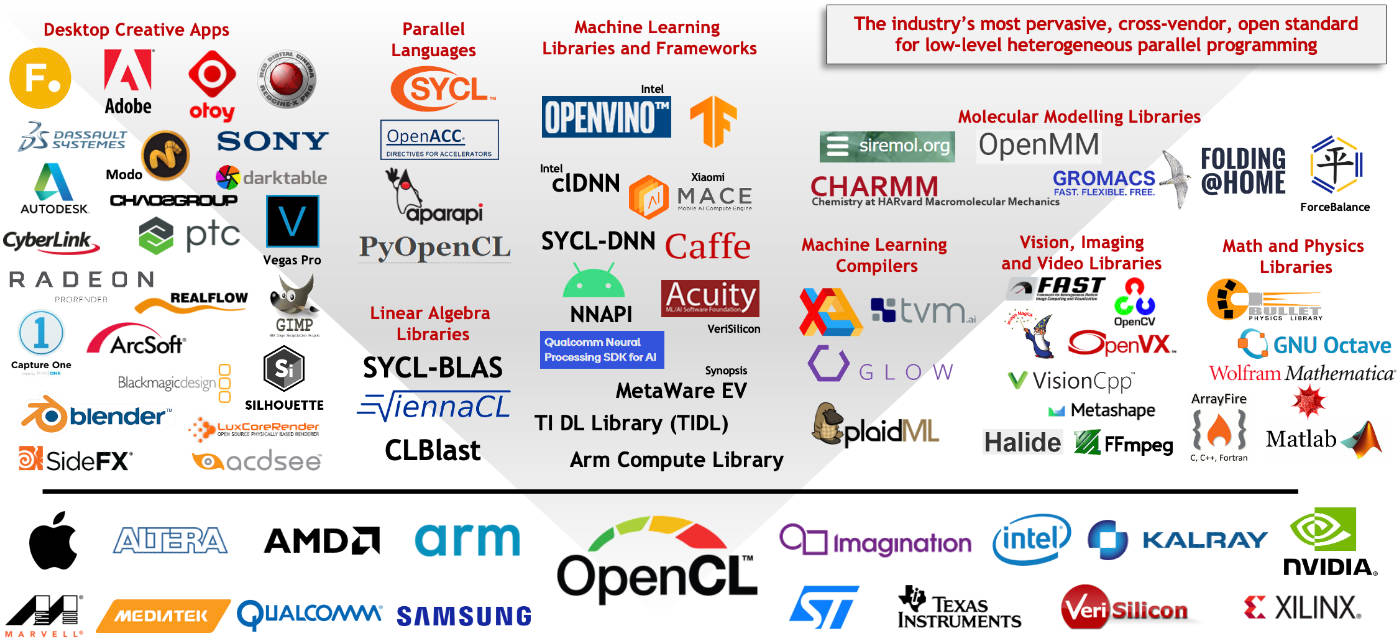
\includegraphics[width=\textwidth]{img/opencl-accelerated-apps.png}
    \captionsetup{justification=centering}
    \caption{OpenCL accelerated applications (Credit: Khronos Group)}
    \label{fig:opencl_accelerated_apps}
\end{figure}

\subsection{EngineCL}
EngineCL \cite{enginecl}, introduces a new object-oriented API on top of OpenCL. The EngineCL class provides a higher level view of the OpenCL context and management of the available devices. The engine in turn uses a Program object which internally manages all the data transfers between the device buffers, the user only needs to provide host input and output buffers, as well as the kernel arguments in order to begin execution. In addition, multiple devices can be used during a single run, the scheduling of which is handled by a Scheduler object. Different scheduling strategies are tested by the paper, with the best results achieved by the HGuided algorithm. HGuided is a dynamic algorithm which starts by assigning big block sizes to all devices and reducing the size of subsequent ones as the execution progresses. This reduces data transfer and synchronization overhead while allowing devices to finish simultaneously towards the end of the execution.

\subsection{FluidiCL}
FluidiCL \cite{fluidicl} maintains the OpenCL API but implements it in such a way that the user can treat multiple devices as a single entity. Thus, it is very easy to adapt an existing OpenCL application to run using FluidiCL, as all function calls can remain unchanged. The paper considers the implementation running on an experimental system with a single GPU and CPU. At the time of setup, both kernel compilation and buffer writes are broadcasted to both devices. That is, the kernel is compiled for both and, likewise, the input data is transferred to both of their buffers. When the execution starts, the GPU starts running the kernel with a decreasing order of work-group IDs, meanwhile the CPU executes smaller sub-kernels in increasing order of work-group IDs. At some point, when the work-groups IDs handled by both cross over, the work is finished and the results are merged on the GPU.

\section{AMD ROCm} \label{sect:rocm}
Initially announced in November 2015 as the "Boltzmann Initiative", AMD ROCm is an open-source software development platform for HPC GPU computing \cite{boltzmann_initiative}. It is AMD's latest competitor to Nvidia's CUDA.

Since shifting their focus away from CTM in 2008 and mainly supporting the OpenCL standard, AMD still lost a significant market share to Nvidia in the GPGPU market \cite{amd_as_alternative}. Developers preferred the CUDA approach which, although constrained them to Nvidia products, provided a more convenient programming experience by following a single source model.

In order to further tap into the GPGPU market, mostly filled by CUDA developers, AMD implemented ROCm and, being more specific, HIP. HIP is a C++ Runtime API and kernel language very similar to CUDA that is portable across Nvidia and AMD GPUs. Porting a CUDA application to HIP does not involve much more than replacing all instances of \textbf{cuda} in the file with \textbf{hip}. AMD also provides the \textit{Hipify} tool, which performs these operations automatically.

HIP code can be compiled for either AMD or Nvidia GPUs. Compilation was previously handled by \texttt{hcc} and \texttt{nvcc} respectively, but these tools have been replaced in ROCm v3.5 by the HIP-Clang compiler, which can compile code for both vendors.

When compared to OpenCL, HIP, like CUDA, has the advantage of a single source C++ programming model. Host and device code can live in the same file and use most of C++'s feature set including lambdas, templates and classes. Thus, porting CUDA code is significantly easier for HIP as mentioned previously. Porting from CUDA to OpenCL not only involves separating device code from host code, it also requires translating this device code from C++ to OpenCL C and modifying all CUDA function calls and keywords to their OpenCL counterparts.

As a case study, in SC16 Ben Sander from AMD made a presentation showing the work required to port CAFFE, a popular machine learning framework with 50,000 lines of CUDA code from CUDA to HIP \cite{caffe_rocm_port}. As shown in figure \ref{fig:caffe-rocm-port}, the HIP port of CAFFE only required changing 907 lines of code (LOC), out of which 688 (almost 76\%) was done automatically. Manual changes to the code took a single developer less than a week to complete. By contrast the OpenCL implementation of CAFFE required changing more than 30,000 LOC.

\begin{figure}[ht]
    \centering
    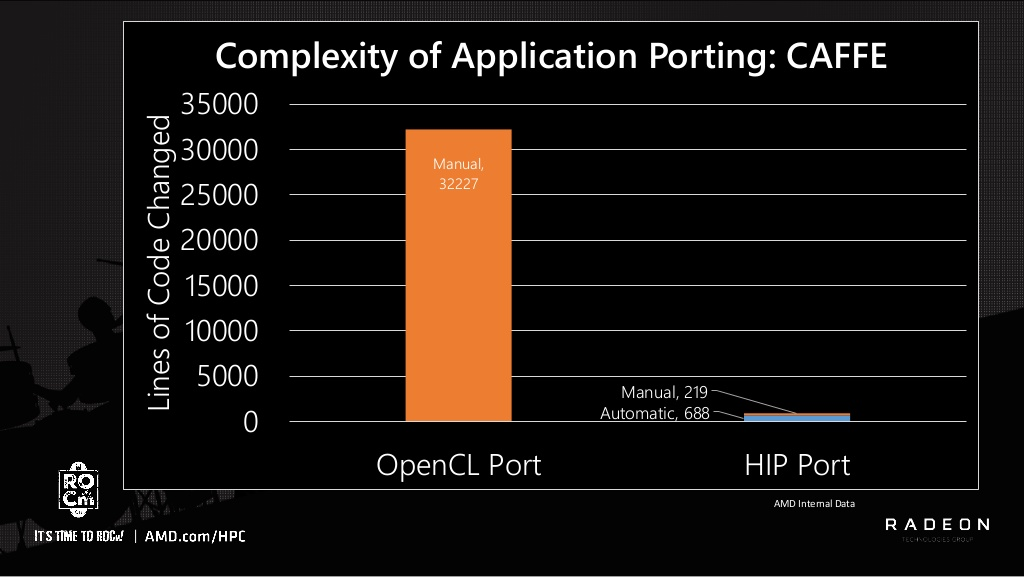
\includegraphics[width=\textwidth]{img/caffe-rocm-port.png}
    \captionsetup{justification=centering}
    \caption{Complexity of porting CAFFE, OpenCL vs HIP (Credit: AMD)}
    \label{fig:caffe-rocm-port}
\end{figure}

\cite{ginkgo_rocm_port} also presents a case of porting an application from CUDA to HIP. Tsai et al. found the process very smooth and were able to automatize most of the work by extending the initial Hipify script to their needs. Although HIP allowed them to run their application on both AMD and Nvidia, they still preferred to keep native support for CUDA and maintain two versions at the same time. This setup allowed them to take advantage of HIP's similarity to CUDA by sharing a third of the code base between both implementations. In the cases where they used CUDA specific functionality, they were able to replicate it in HIP and use a common API to call the appropriate implementation depending on the programming model used. Finally, they also included experiments to show the performance of HIP code compared to native CUDA on Nvidia GPUs. These tests showed that the overhead of HIP over CUDA is negligible, with 50\% of the test cases showing less than 3\% performance difference and 90\% of the test cases showing less than 10\% performance difference.

\section{OpenMP \& OpenACC} \label{sect:openmp-openacc}
In this section we will tackle OpenMP and OpenACC in conjunction as they take very similar approaches.

Both projects are composed of a library and set of compiler directives that provide a model for parallel programming across different architectures. Support is provided for the C, C++ and Fortran languages. The directives extend the languages with useful constructs for parallelizing applications. Further control of the runtime environment is possible through the library \cite{openmp_spec, openacc_spec}.

OpenMP and OpenACC allow for quick adaptation of existing single threaded code into a parallel execution model. This work requires a compiler which supports the standard, meaning that it is able to handle the directives and generate multithreaded code automatically.

An example of offloaded OpenMP code can be seen in listing \ref{lst:openmp_saxpy}. The code looks like a regular serial implementation of SAXPY for a general purpose processor, except for the two \texttt{\#pragma}s. The first pragma instructs OpenMP to offload the following code onto an accelerator, and specifies which variables must be copied \textbf{to} the accelerator when entering the scope (a, x and y) and which must be copied \textbf{from} the accelerator when leaving the scope (only z). The second pragma indicates that the for loop can be executed in parallel, that way the compiler can be sure that all operations are independent and capable of running in separate threads.

\begin{lstlisting}[style=CStyle, caption=OpenMP saxpy example, float, floatplacement=H, label={lst:openmp_saxpy}]
int main(void) {
    float a;
    float x[100], y[100], z[100];

    // Omitted: Initialize a, x, y

    #pragma omp target map(to:a, x[0:100], y[0:100]) map(from:z[0:100])
    #pragma omp parallel for
    for (int i = 0; i < 100; i++) {
        z[i] = a * x[i] + y[i];
    }
}
\end{lstlisting}

Up until version 4.0, OpenMP only allowed this code to be compiled for and executed on the CPU. Version 4.0 (2013) introduced offloading of parallel code onto other devices, like GPUs or FPGAs \cite{openmp_gpu_support}. Meanwhile, OpenACC focused on heterogeneous computing and accelerator offloading from the start \cite{openacc_initial_spec}, also treating the multicore CPU itself as a device.

\cite{openmp_vs_openacc} provides a comparison of both programming models in terms of programmability and expressiveness. Here the authors denote the differences between OpenMP and OpenACC when implementing common parallel programming patterns targeting accelerators. Overall, the resulting code and directives used are mostly equivalent, with OpenACC having a slight advantage thanks to providing accelerator support since its inception. In terms of programmer effort, there is no significant difference. In terms of performance however, \cite{cuda_openacc_openmp_performance} shows that the code generated by OpenACC is able to utilize more memory bandwidth and thus perform better than OpenMP, specially when using a naïve approach. Still, both approaches fall behind a pure CUDA kernel.

Finally, the possibility to use both models at the same time exists. Works like \cite{openmp_openacc_multigpus} exploit parallelism on the CPU with OpenMP to schedule code to run on multiple GPUs. \cite{openmp_openacc_molecular_docking} also leverages this hybrid approach to run kernels which are more GPU friendly on the GPU using OpenACC while running less friendly kernels with OpenMP CPU parallelization.

\section{SYCL} \label{sect:sycl}
SYCL \cite{sycl_2020_standard} is a C++ programming model for heterogeneous computing. It builds on the underlying concepts, portability and flexibility of parallel APIs or standards like OpenCL while adding the ease of use and flexibility of single-source C++. Initially, SYCL was released as OpenCL SYCL with a provisional specification in 2014, and acted as a higher level API to interact with OpenCL devices. Since the newest SYCL 2020 standard, the model has become more generalized, making OpenCL just one of the different potential programming models SYCL can be based upon \cite{sycl_faq}.

In SYCL, device and host code live on the same file and can be written in C++ according to the C++17 standard (ISO/IEC 14882:2017 Programming languages — C++) \cite{cpp17} and also the newest C++20 standard (ISO/IEC 14882:2020 Programming languages — C++) \cite{cpp20}. For compatibility reasons, the entire set of C++ features is not available in device code. In particular, SYCL device code does not support virtual function calls, function pointers, exceptions, runtime type information or dynamic memory allocation.  This still leaves a big portion of the standard which is compatible with host and device code alike, allowing the reuse of types, library code, templates and abstractions. In addition, the programmer does not need to switch between languages depending which part of the code base they are modifying. It is also important to note that, as long as there is no dependencies created with the underlying SYCL implementation, a standard C++ compiler can compile SYCL programs to run directly on the host CPU, without any external accelerator.

To facilitate integration, SYCL is designed to allow each source file to be passed through multiple different compilers, the outputs of which are combined into a single source file. The programmer can then add SYCL code to an existing project and continue using their preferred host compiler while the SYCL tools handle compilation for the device code.

An example SYCL code snippet can be seen in listing \ref{lst:sycl_saxpy}.

\begin{lstlisting}[style=CStyle, caption=SYCL saxpy example, float, floatplacement=H, label={lst:sycl_saxpy}]
using namespace sycl;
float A;
float h_X[100], h_Y[100], h_Z[100];

// Omitted: Initialize A, h_X, h_Y

queue q; // Queue to enqueue work to the default device

// Wrap the arrays in buffers
buffer<float,1> d_X { h_X, range<1>(100) };
buffer<float,1> d_Y { h_Y, range<1>(100) };
buffer<float,1> d_Z { h_Z, range<1>(100) };

q.submit([&](handler& h) {
    auto X = d_X.get_access<access::mode::read>(h);
    auto Y = d_Y.get_access<access::mode::read>(h);
    auto Z = d_Z.get_access<access::mode::read_write>(h);

    // Enqueue a parallel_for task with 100 work-items executing the saxpy kernel
    h.parallel_for(100, [=] (id<1> idx) {
        Z[idx] = A * X[idx] + Y[idx];
    });
});
q.wait();
\end{lstlisting}

The code within the the lambda argument to the \texttt{parallel\_for} is the device kernel. This code will be compiled using the device compiler and executed on the device.

SYCL can be laid out on top of multiple backends. A backend exposes one or multiple SYCL platforms (collections of devices). For example, implementations can expose an OpenCL backend to give access to OpenCL devices, or a CUDA backend to give access to Nvidia GPUs. Apart from the generic API that all backends must implement in order to provide the basic device functionality, each backend can expose their specific features through interoperability headers to provide the developer with more control at the expense of portability.

When building a SYCL application, the user can choose which backends to use. This is the set of \textit{active backends} for the application. The application can then be run on any host platform that supports at least one of the active backends. The subset of active backends which are supported by the host platform at runtime are called the \textit{available backends}.

A diagram with the SYCL implementations in development and their provided backends can be seen in figure \ref{fig:sycl-implementations}. As shown, the available SYCL implementations cover a wide range of hardware. As long as the programmer does not use any backend-specific feature, their application can be executed in any available implementation without modifications.

\begin{figure}[ht]
    \centering
    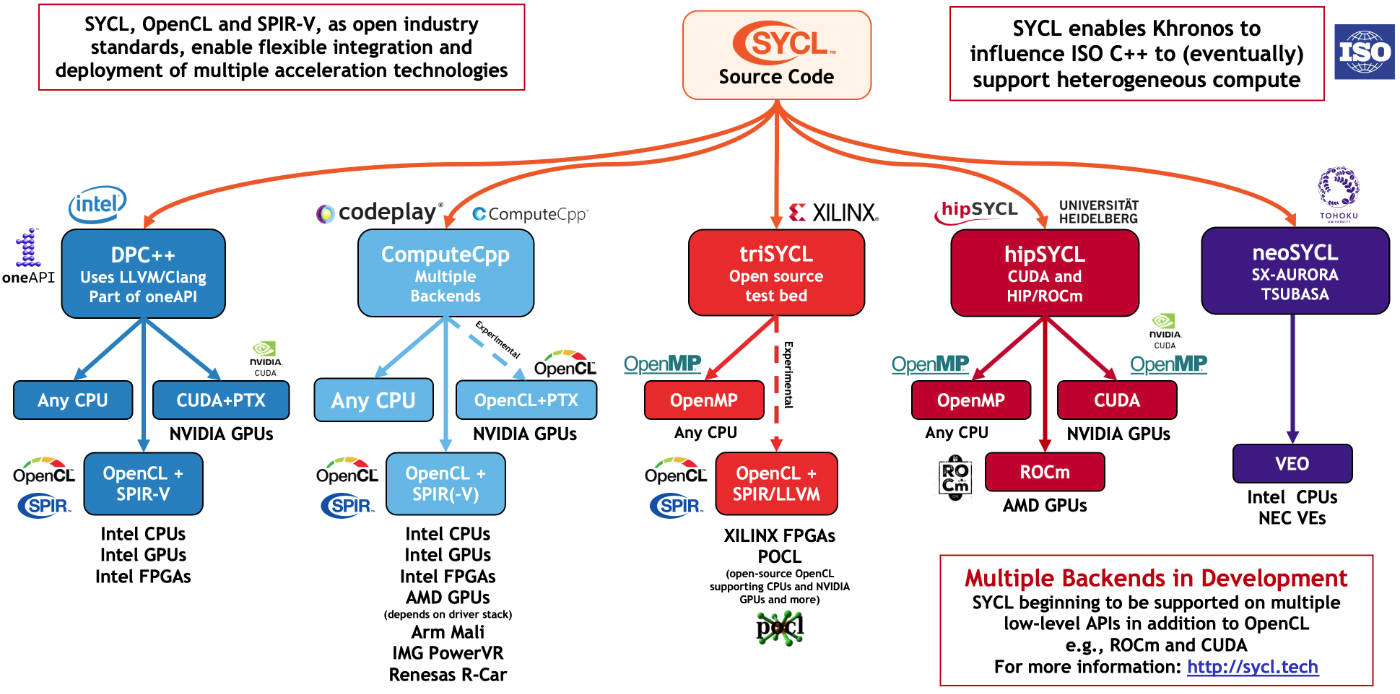
\includegraphics[width=\textwidth]{img/sycl-implementations.png}
    \captionsetup{justification=centering}
    \caption{SYCL implementations in development (Credit: Khronos Group)}
    \label{fig:sycl-implementations}
\end{figure}

In \cite{performance_portability_multimaterial_kernels} Reguly studies the performance of multiple different programming models on both CPUs and GPUs. These programming models include: OpenMP, OpenACC, CUDA, SYCL and Kokkos (covered in the following section). In the paper, two multi-material simulation problems are used as benchmarks. In multi-material simulations, each cell in the simulation domain can have one or multiple different materials. Given these multi-material cells, the three algorithms used to solve the proposed benchmark problems compute the density and pressure of each material over each cell and their neighboring cells. Performance is measured in terms of fraction of peak performance, where peak performance is the theoretical maximum memory bandwidth possible for each device. In GPUs, SYCL (in particular the hipSYCL implementation) is able to achieve very similar results to pure CUDA kernels, the best performing model, in both problems. The situation is different when looking at CPUs, where SYCL implementations are 5-15\% slower than OpenMP ones.

\cite{sycl_hpc_applications} presents a more recent survey of SYCL performance. It evaluates the memory bandwidth achieved by three different applications:
\begin{itemize}
    \item BabelStream: A popular measure of memory transfer speeds to and from global device memory.
    \item Heat: 5-point stencil which computes the weighted average between a cell and its four neighbors.
    \item CloverLeaf: Largest application in the group, with close to 8,000 lines of code. It is composed of around 11 routines, each one performing either point-wise or stencil updates over a 2D grid.
\end{itemize}
All these applications are memory bandwidth bound, as it is common in HPC applications today.
In this study, SYCL proved to incur in very little overhead over the underlying implementations. Any performance problems shown in the applications were also reproduced in the direct implementations for the underlying programming models, so they are not SYCL level issues. What this study shows is that there is a clear need for better vendor support. All GPU implementations rely on open source projects which do not offer commercial support from the hardware vendors. Also, as SYCL is currently mostly built on top of other programming models, it relies on the maturity and support of their implementations as well.

\subsection{Celerity}
Celerity \cite{celerity} is an API for programming distributed memory accelerator clusters. It is built on top of SYCL and extends its programming model, allowing the user to distribute the work and data across multiple nodes in an automatic way. Celerity also leverages MPI (Message Passing Interface) \cite{mpi} to enable inter-node communication.

The Celerity extensions act as a wrapper over the SYCL runtime, handling inter-node communication and scheduling, while each individual node executes the SYCL kernel in parallel. In order to enable this, Celerity introduces a global distributed queue, replacing the device local queues of SYCL. It also adds the requirement to specify the data access of each kernel, for reading and writing to the buffers. This allows Celerity to know beforehand which pieces of data need to be present at each node when distributing the work, and also to reconstruct the output buffer when the execution finishes.

Celerity's execution model is arranged in a master/worker fashion. Each worker node encapsulates the available accelerator hardware and receives commands coming from a master node, which is responsible for scheduling the work. In order to construct a dependency graph of the kernels to execute, the Celerity runtime executes the programs twice. First, in the \textit{pre-pass}, information about the kernel is collected, this includes buffer accesses, how these accesses are mapped into outputs, and the global size of the kernel. With this data, the master can construct the graph and generate commands to distribute to the workers. These commands not only contain buffer data and the kernel function, but also dependency information. This allows the workers to perform peer-to-peer communication during the \textit{live-pass} as necessary and start execution as soon as their dependencies are fulfilled, instead of requiring communication with the master at each instance. This means that Celerity does not induce any extra bandwidth overhead compared to a fully decentralized approach.

\section{Kokkos} \label{sect:kokkos}
Kokkos \cite{kokkos} is a C++ library that enables applications and domain libraries to achieve performance portability on manycore architectures by unifying abstractions for both fine-grain data parallelism and memory access patterns.

As a library-only solution, Kokkos does not require external tools such as a specialized compiler or even compiler extensions. Kokkos can be linked as a regular C++ library with CMake.

One of the main features provided by this programming model, and the one that distinguishes it from the rest, are \texttt{View} objects. \texttt{View}s are used as storage for kernel computations. Instead of using raw pointers and arrays, where the indexing is done as a simple memory reference at a given offset, \texttt{View}s change their memory layout depending on the device the kernel is running on. Operations on a \texttt{View} are not affected at all by this change, allowing kernels to be portable across devices while also providing the optimal memory access pattern on each architecture.

To implement parallelism, Kokkos provides a set of functions that cover different \textit{Execution Patterns}. These include parallel loops with \texttt{parallel\_for}, reductions with \texttt{parallel\_reduce}, scans with \texttt{parallel\_scan} and spawning of individual tasks. These patterns can also be nested, for example one can execute a \texttt{parallel\_reduce} inside a \texttt{parallel\_for} or vice versa.

Kokkos is built on top of multiple backends. This means that it is not tied to any particular underlying implementation and can use the best performing programming model available on a particular platform. These backends include OpenMP, CUDA, ROCm, HPX \cite{hpx}, SYCL and pthreads.

In terms of performance, the initial implementation presented in \cite{kokkos} showed it was capable of achieving at least 90\% of the performance of the architecture specific, optimized variants of the same benchmarks (i.e. comparing Kokkos against OpenMP for CPUs and CUDA for GPUs). \cite{performance_portability_multimaterial_kernels} also evaluates the performance of Kokkos. As mentioned in the SYCL section, this paper uses two different multi-material problems as benchmarks. The overall performance of Kokkos is 6\% lower for the first problem and 22\% lower for the second problem. While CUDA and OpenMP implementations have the advantage, they also require different codebases, while Kokkos is completely portable across devices.


\section{MANGO V1} \label{sect:mangov1}
The first version of the MANGO project, here referenced to as MANGO V1, presents a programming model that simplifies the development of parallel applications exploiting deeply heterogeneous architectures. 

Providing a C and a C++ API, what separates MANGO from the previously mentioned alternatives is the inclusion of a resource manager (BarbequeRTRM \ref{bbque}). The resource manager is capable of scheduling user's tasks over the system available accelerators according to user requirements and the current state of the system. 
A custom hardware architecture, consisting on multiple clusters of FPGA accelerators, and capable of fast reconfiguration, was developed along the MANGO software stack and utilized for the exploration of manycore architectures for HPC systems.
As a result, MANGO V1 offers support for PEAK, nu+ and DCT accelerators, while also providing CPU emulation of these, for development and testing purposes.

\begin{lstlisting}[style=CStyle, caption=MANGO saxpy example (host), floatplacement=H, label={lst:mangov1_sample}]
#define KERNEL 1
#define B1 1
#define B2 2
#define B3 3

int main(int argc, char const *argv[])
{
    // Initialization
    mango::mango_init_logger();
    auto mango_rt = mango::Context("gn_saxpy", "test_manga");

    // Omitted: Initialize a, n, x, y, o

    char kernel_path[] = "/opt/mango/usr/local/share/gn_saxpy/saxpy";
    auto kf = std::make_shared<mango::KernelFunction>();
    kf->load(kernel_path, mango::UnitType::GN, mango::FileType::BINARY);

    // Register task graph
    auto k  = mango_rt.register_kernel(KERNEL, kf, {B1, B2}, {B3});
    auto b1 = mango_rt.register_buffer(B1, buffer_size, {}, {KERNEL});
    auto b2 = mango_rt.register_buffer(B2, buffer_size, {}, {KERNEL});
    auto b3 = mango_rt.register_buffer(B3, buffer_size, {KERNEL}, {});

    auto tg = mango::TaskGraph({k}, {b1, b2, b3});

    // Resource Allocation
    mango_rt.resource_allocation(tg);

    // Set up arguments
    auto argX = mango::BufferArg(b1);
    auto argY = mango::BufferArg(b2);
    auto argO = mango::BufferArg(b3);
    auto argA = mango::ScalarArg<float>(a);
    auto argN = mango::ScalarArg<int>(n);

    auto argsKERNEL = 
        mango::KernelArguments({argA, argX, argY, argO, argN}, k);

    // Omitted: Write to buffers

    // Start kernel
    auto e = mango_rt.start_kernel(k, argsKERNEL);

    // Wait for kernel termination
    e->wait();

    // Omitted: Check results and free resources
}
\end{lstlisting}

Mainly due to its resource management capabilities, MANGO's programming model provides a level of abstraction over the hardware far greater than its competition, removing the querying of platform information from the list of user responsibilities. 
As seen in listing \ref{lst:mangov1_sample}, the only architecture specific information required is a kernel compatible with its target accelerator. Multiple kernel versions can be provided for a single task, leaving to the resource manager the decision of which accelerator performs its execution. 

MANGO's API exposes a set of data structures for the specification of an user's application. A \texttt{TaskGraph} holds \texttt{Kernel}, \texttt{Buffer} and \texttt{Event} data structures, defining their dependencies. 
Once the task graph is defined, the resource allocation is performed.
Kernel termination events are automatically generated for synchronization purposes, while users can specify custom events to use as desired.
A variety of kernel arguments are supported, including scalar values, memory buffers and user events. Arguments are grouped in a \texttt{KernelArguments} structure, which is passed when a kernel is started.

MANGO V1 was the foundation for our work, in which we seek to further improve the platform through a number of additions that help close gaps left by other solutions in this field.

\section{Gap Analysis}

In this section, we will compare the programming models seen so far in order to analyze the present gaps in the heterogeneous computing space that MANGO can fill.
As explained previously, MANGO is an ongoing project with the goal of enabling the development of user applications on heterogeneous HPC systems, while including a system resource manager. 
Our contributions to the project focused on the addition of a Python language API, Just In Time compilation of kernels, and GPU support.
This work resulted in a new version of the system: MANGO V2.

For the following analysis, we consider MANGO V1 and MANGO V2 separately to further differentiate the capabilities that were already present in the first version of the system, from those introduced by our contributions.

The capabilities we are interested in for the presented programming models are:

\begin{itemize}
    \item Device support, including CPU, GPU and FPGAs.
    \item Whether the model uses a single-source approach, where host and device code can coexist in the same source file, are written in the same programming language and can share common pieces of code.
    \item The portability of the device kernels, as in whether it is possible for a kernel written to target a given device to be compiled for and executed in a different supported device.
    \item The ability to compile kernels at runtime (Just In Time compilation), according to their target accelerators.
    \item Resource management capabilities, allowing efficient use of the available devices depending on their current load, power consumption and relative performance.
    \item Support for control and distribution of the application along multiple clusters, each one with a set of diverse target devices.
\end{itemize}

A comparison of the capabilities of each programming model can be seen in table \ref{tab:progamming-model-comparison}.

%TODO explain stars
\begin{table}[ht]
    \centering
    \begin{tabular}{l|c|c|c|c|c|c|c|c}
    \textit{Model} & \textit{CPU} & \textit{GPU} & \textit{FPGA} & \makecell{\textit{Single} \\ \textit{source}} & \makecell{\textit{Kernel} \\ \textit{portability}} & \makecell{\textit{Kernel JIT} \\ \textit{compilation}} & \makecell{\textit{Resource} \\ \textit{management}} & \makecell{\textit{Multiple} \\ \textit{clusters}} \\ \hline
    MANGO V1 & Yes* & No & Yes & No & No & No & Yes & Yes* \\
    MANGO V2 & Yes & Yes & Yes* & No & No & Yes & Yes & Yes* \\
    CUDA & No & Yes & No & Yes & No & No & No & No \\
    OpenCL & Yes & Yes & Yes & No & Yes & Yes & No & No \\
    EngineCL & Yes & Yes & Yes & No & Yes & Yes & No & No \\
    FluidiCL & Yes & Yes & Yes & No & Yes & Yes & No & No \\
    ROCm & No & Yes & No & Yes & Yes & No & No & No \\
    OpenMP & Yes & Yes & No & Yes & Yes & No & No & No  \\
    OpenACC & Yes & Yes & No & Yes & Yes & No & No & No  \\
    SYCL & Yes & Yes & Yes & Yes & Yes & No & No & No \\
    Celerity & Yes & Yes & Yes & Yes & Yes & No & No & Yes \\
    Kokkos & Yes & Yes & No & Yes & Yes & No & No & No 
    \end{tabular}
    \captionsetup{justification=centering}
    \caption{Comparison of programming model capabilities}
    \label{tab:progamming-model-comparison}
\end{table}

In MANGO V2, GPUs were added to the pool of supported accelerators, and CPU devices are now handled independently (in the previous version, CPU and FPGA usage was mutually exclusive).
As part of our work, we introduced a new module named Heterogeneous Hardware Abstraction Layer (HHAL) \ref{HHAL}, capable of handling communication with multiple target accelerators and providing an easy path for integrating new devices.

By looking at the table, we can see that there are two capabilities still not covered by MANGO V2: it is not a single source approach and also requires writing a separate kernel for each device.

We argue that, although at first glance introducing these capabilities would improve programmability, the performance gained by their absence is much more important to HPC.

First of all, using a single kernel programming model for multiple devices, even one that is open source, does not guarantee portability. We will take OpenCL as an example. As seen in section \ref{sect:opencl}, it is the responsibility of the hardware vendors to provide support for any new feature of the standard. This introduces version differences between different platforms, for example Nvidia GPUs still only support OpenCL 1.2. While OpenCL 2.x introduced multiple useful features, the lack of support from Nvidia, which is one of its main targets, slowed down 2.0 adoption. The effect was so considerable that the 3.0 standard removed the requirement for most of the features introduced in 2.x. 

If a developer has two target OpenCL devices for the same kernel, one with 1.2 capabilities and one with 2.0 capabilities one of two things can happen: 
\begin{enumerate}
    \item they limit themselves to 1.2 features, or
    \item they write two separate kernels and possibly two separate host side implementations to exploit all the newest features on the device that supports the latest standard, while also maintaining compatibility with the 1.2 device.
\end{enumerate}
 
As such, a great hurdle for kernel portability is the hardware vendors' unwillingness to work together \cite{but_mummy_cuda}. This is perfectly reasonable, like in any other market, a company will gain an advantage over their competitors in whichever way they can and maintain it as long as possible. If Nvidia simply releases CUDA as an open source standard for all GPUs to utilize, they will lose their upper hand over AMD in the GPGPU market.

Even if, despite all their differences, all hardware vendors would work together on a single project, the differences in the hardware architecture will still be present. Indeed, the purpose of Heterogeneous Computing is to handle multiple devices with different memory access requirements, levels of parallelism, instruction sets and more. Although it may be possible to abstract all this away from the kernel programmer, it will not come without a cost in performance.

In order to squeeze all the performance out of the devices it is necessary to use a low-level language which takes into account the specific details of the hardware \cite{cuda_open_source_compiler}. This does not mean that all kernels have to be written in assembly, but in a language that makes it possible to utilize all the capabilities offered by the target device. In consequence, it is inevitable that one or more of the available devices do not present a given capability. Thus, in today's world, achieving complete portability of a kernel while also maintaining peak performance is impossible.

MANGO's plan is to embrace these differences in kernel implementations, allowing the developers to write their device code in the best suited programming language or framework available. Our programming model abstracts away all the \textit{host side} code to be able to handle multiple different platforms, allowing for different types of implementations to coexist and communicate with each other, no matter what the chosen model for the device kernel is.

A rarely supported functionality is Just In Time compilation of kernels. With OpenCL and its users being the only ones to provide run-time compilation of kernels, in MANGO V2 we introduced, as part of the HHAL module, a Dynamic Compiler \ref{HHAL:DynamicCompiler}. The Dynamic Compiler is capable of compiling kernels at run-time for each of the supported devices, this way kernels are compiled from source as needed, according to their assigned accelerator.
The main advantage this functionality gives is smoothing the development process, by allowing developers to work directly with kernel source code without requiring manual compilation for each target architecture.

The key advantage of MANGO over the other mentioned programming models is its integration with a resource manager, namely BarbequeRTRM \ref{bbque}. While the previous models focus on executing a single kernel or set of kernels as fast as possible on a given platform, they do not take into account the current state of the machine that they are running on. If multiple applications could be running at the same time, there is a chance that the device most suitable for a given application is currently busy serving something else. Depending on what other devices are available, their relative performance for the kernel, power consumption and other aspects, it may be more efficient to execute the work on a different device or just wait for the preferred one to be available. In addition, it could also be advantageous to suspend the execution of a given application in order to give priority to another which is more time sensitive.

Lastly, no other model except Celerity offers distributed execution of an application over multiple clusters. Since its inception, one of the goals of MANGO was to provide this capability, allowing it to exploit the heterogeneity of a large number of different machines. In conjunction with Barbeque, which also provides the capability to manage resources in a distributed system, it would be possible to launch a number of different applications on a multitude of computers and achieve an efficient and performant execution of all tasks. There are still advancements to be done in this front, as it was not the topic of our work, but many implementation decisions were driven by it.